% =============================================================================
% PART B - MODULE 15 (15.01 - 15.03): ADMINISTRATOR MASTER DATA CATALOGS
% In Charge: Nguyen Tien Thuan (CE181024)
% =============================================================================

\newpage
\subsection{Module 15: Administrator Master Data Catalog Management}

The Administrator Master Data Catalog Management module empowers system administrators to maintain foundational classification dictionaries across \textbf{Frevia}, including: Technical Skills catalogs (\textbf{Skills}), Job \& Industry categories (\textbf{Job Categories}), and Community Forum topic boards (\textbf{Forum Categories}). To maintain data integrity across active job postings, freelancer portfolios, and historical community discussions, all catalog items utilize a non-destructive \textbf{Soft Delete and Restore} lifecycle architecture.

% -----------------------------------------------------------------------------
\subsubsection{M15.01 -- Skills Catalog Management with Soft Delete \& Restore (UC-11.01 to UC-11.06)}

\begin{itemize}[leftmargin=1.5em,itemsep=2pt]
  \item \textbf{Screen Name \& Route Path:} Skills Management Console -- \texttt{/admin/skills}.
  \item \textbf{Target Actor:} Administrator.
  \item \textbf{Preconditions:} Administrator has permissions to access the \texttt{ADMIN\_SKILLS} module.
\end{itemize}

\begin{figure}[H]
  \centering
  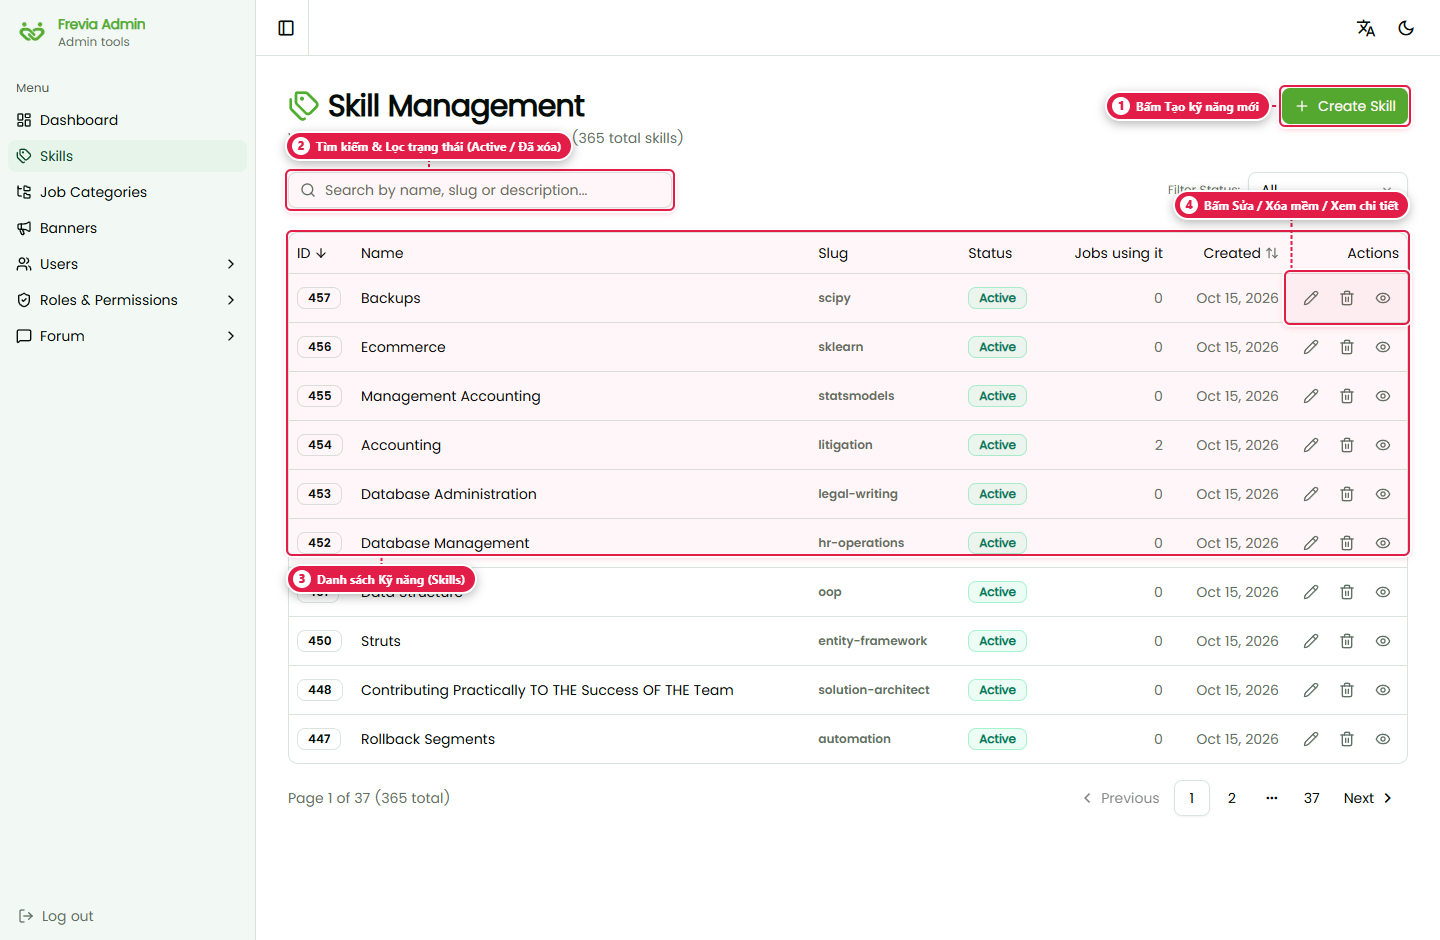
\includegraphics[width=0.90\textwidth]{images/admin/m15_01_admin_skills.png}
  \caption{Skills catalog management console with search and soft delete at \texttt{/admin/skills}}
\end{figure}

\paragraph{Step-by-Step User Instructions:}
\begin{enumerate}[leftmargin=1.8em,itemsep=3pt]
  \item In the Admin sidebar, click \textbf{Skills}.
  \item \rbadge{1} \textbf{Create New Skill (\textit{+ Create Skill}):} Click the blue \textbf{+ Create Skill} button in the top right to open the creation dialog (specify Skill Name, auto-generated or custom Slug, and Description).
  \item \rbadge{2} \textbf{Search and Filter Skills (\textit{Search \& Status filter}):} Type a query into the \textit{Search by name, slug or description...} box, or select a status from \textit{Filter Status} (\textit{All}, \textit{Active}, or \textit{Deleted}).
  \item \rbadge{3} \textbf{Inspect Skills Data Table (\textit{Skills Table}):} Review catalog rows displaying \textit{ID}, \textit{Name}, \textit{Slug}, \textit{Status} badge (\textbf{Active} or \textbf{Deleted}), \textit{Jobs using it} tally, and \textit{Created} date.
  \item \rbadge{4} \textbf{Perform Row Actions (\textit{Actions column}):}
    \begin{itemize}
      \item Click the pencil icon (\textbf{Pencil icon}) to edit skill attributes.
      \item Click the trash icon (\textbf{Trash icon}) to execute a \textbf{Soft Delete}. For previously deleted skills (indicated by a red \textbf{Deleted} badge), this button transforms into a circular restore icon (\textbf{Restore icon}), allowing the administrator to reactivate the skill back to \textbf{Active} status.
      \item Click the eye icon (\textbf{Eye icon}) to view detailed skill metrics at \texttt{/admin/skills/[id]}.
    \end{itemize}
\end{enumerate}

\paragraph{Expected Output \& Exception Handling:}
\begin{itemize}[leftmargin=1.5em,itemsep=2pt]
  \item \textbf{Success Scenario:} Newly added or updated skills become available immediately in the autocomplete suggestions for client job postings and freelancer profiles. Soft deletion sets \texttt{deletedAt = NOW()} without breaking existing foreign key associations.
  \item \textbf{Exception Scenarios:} If a user attempts to create a skill with a duplicate Name or Slug, the server rejects the request with an explicit uniqueness validation error.
\end{itemize}

% -----------------------------------------------------------------------------
\newpage
\subsubsection{M15.02 -- Job Categories \& Industry Classification Management (UC-12.01 to UC-12.06)}

\begin{itemize}[leftmargin=1.5em,itemsep=2pt]
  \item \textbf{Screen Name \& Route Path:} Job Category Management Console -- \texttt{/admin/job-categories}.
  \item \textbf{Target Actor:} Administrator.
  \item \textbf{Preconditions:} Administrator has permissions to access \texttt{ADMIN\_JOB\_CATEGORIES}.
\end{itemize}

\begin{figure}[H]
  \centering
  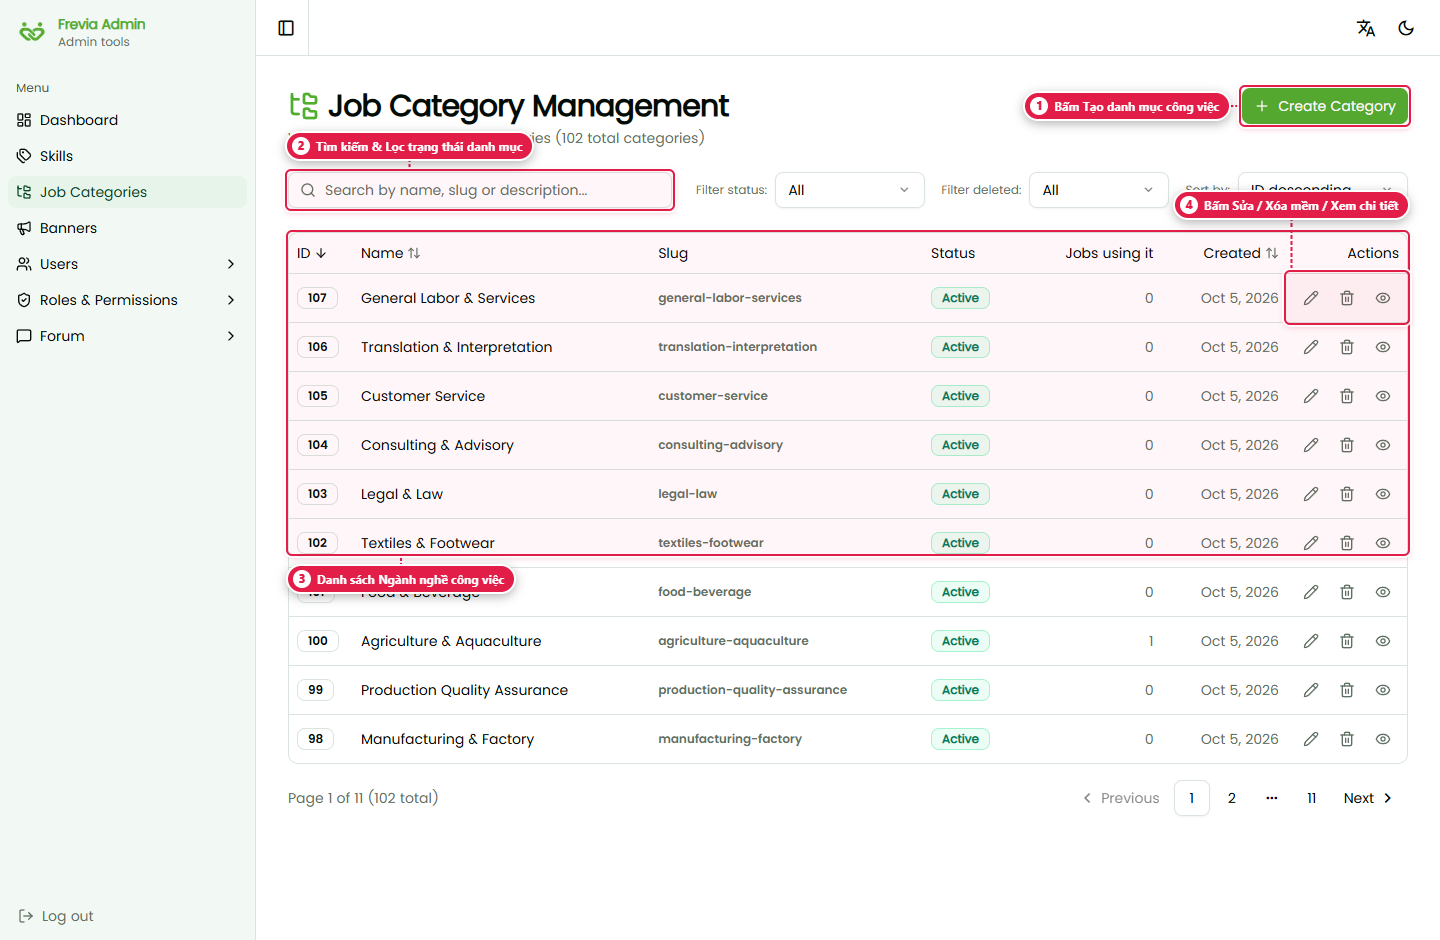
\includegraphics[width=0.90\textwidth]{images/admin/m15_02_admin_job_categories.png}
  \caption{Job Categories management console with category hierarchy at \texttt{/admin/job-categories}}
\end{figure}

\paragraph{Step-by-Step User Instructions:}
\begin{enumerate}[leftmargin=1.8em,itemsep=3pt]
  \item In the Admin sidebar, click \textbf{Job Categories}.
  \item \rbadge{1} \textbf{Create New Job Category (\textit{+ Create Category}):} Click \textbf{+ Create Category} to open the category creation dialog (specify Category Name, Slug, Description, and Icon).
  \item \rbadge{2} \textbf{Search and Status Filter (\textit{Search \& Filter}):} Filter categories by keyword or lifecycle state (\textit{All}, \textit{Active}, \textit{Deleted}).
  \item \rbadge{3} \textbf{Inspect Job Categories Table (\textit{Categories Table}):} Examine records displaying \textit{ID}, \textit{Category Name}, \textit{Slug}, \textit{Description}, \textit{Status}, and associated \textit{Jobs Count}.
  \item \rbadge{4} \textbf{Category Actions (\textit{Actions column}):} Click the pencil icon to update category details, or click the trash/restore icon to perform soft-delete or restore operations.
\end{enumerate}

\paragraph{Expected Output \& Exception Handling:}
\begin{itemize}[leftmargin=1.5em,itemsep=2pt]
  \item \textbf{Success Scenario:} Updated job categories immediately update the marketplace search facets and job creation forms.
\end{itemize}

% -----------------------------------------------------------------------------
\newpage
\subsubsection{M15.03 -- Forum Discussion Categories Management (UC-13.01 to UC-13.06)}

\begin{itemize}[leftmargin=1.5em,itemsep=2pt]
  \item \textbf{Screen Name \& Route Path:} Forum Category Management Console -- \texttt{/admin/categories}.
  \item \textbf{Target Actor:} Administrator.
  \item \textbf{Preconditions:} Administrator has permissions to access \texttt{ADMIN\_FORUM\_CATEGORIES}.
\end{itemize}

\begin{figure}[H]
  \centering
  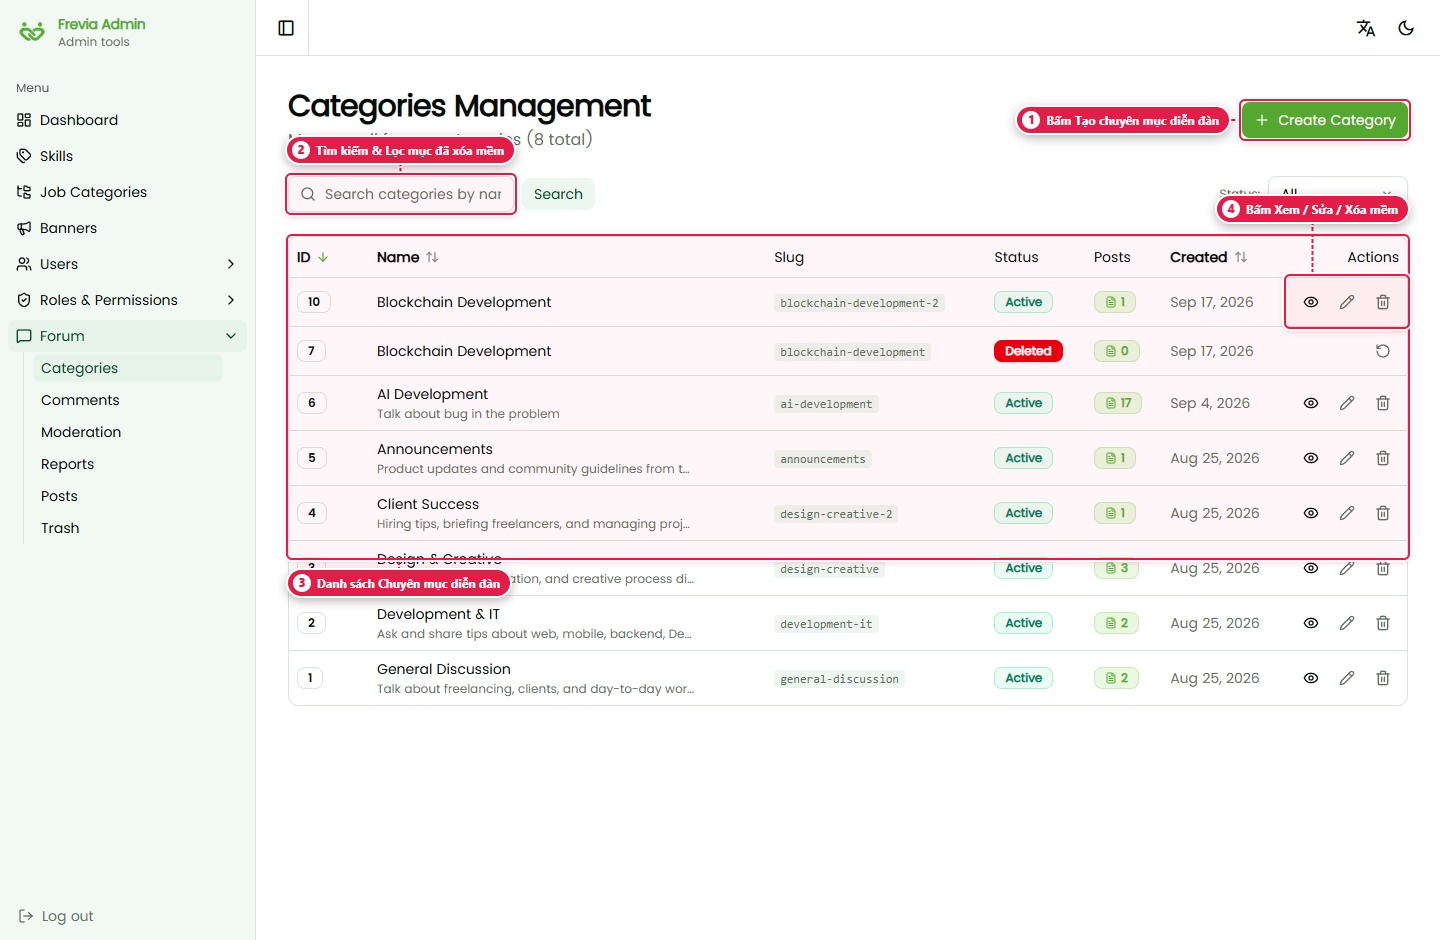
\includegraphics[width=0.90\textwidth]{images/admin/m15_03_admin_forum_categories.png}
  \caption{Forum Discussion Categories management console at \texttt{/admin/categories}}
\end{figure}

\paragraph{Step-by-Step User Instructions:}
\begin{enumerate}[leftmargin=1.8em,itemsep=3pt]
  \item In the Admin sidebar, navigate to \textbf{Forum} $\rightarrow$ \textbf{Categories} (\texttt{/admin/categories}).
  \item \rbadge{1} \textbf{Create New Forum Category (\textit{+ Create Category}):} Click \textbf{+ Create Category} to open the creation dialog (enter Category Name, Slug, Description, and display order).
  \item \rbadge{2} \textbf{Search Forum Categories (\textit{Search input}):} Filter community boards by keyword in real time.
  \item \rbadge{3} \textbf{Inspect Forum Boards Table (\textit{Forum Categories Table}):} View category attributes including \textit{ID}, \textit{Category Name}, \textit{Slug}, \textit{Topics / Posts Count}, and \textit{Status}.
  \item \rbadge{4} \textbf{Manage Forum Categories (\textit{Actions column}):} Use the action icons to edit category details, archive inactive boards via soft-delete, or restore previously archived boards.
\end{enumerate}

\paragraph{Expected Output \& Exception Handling:}
\begin{itemize}[leftmargin=1.5em,itemsep=2pt]
  \item \textbf{Success Scenario:} Community discussion boards on \texttt{/forum} update in real time based on active category configurations.
\end{itemize}
